% ****** Start of file apssamp.tex ******
%
%   This file is part of the APS files in the REVTeX 4.1 distribution.
%   Version 4.1r of REVTeX, August 2010
%
%   Copyright (c) 2009, 2010 The American Physical Society.
%
%   See the REVTeX 4 README file for restrictions and more information.
%
% TeX'ing this file requires that you have AMS-LaTeX 2.0 installed
% as well as the rest of the prerequisites for REVTeX 4.1
%
% See the REVTeX 4 README file
% It also requires running BibTeX. The commands are as follows:
%
%  1)  latex apssamp.tex
%  2)  bibtex apssamp
%  3)  latex apssamp.tex
%  4)  latex apssamp.tex
%
\documentclass[%
 reprint,
%superscriptaddress,
%groupedaddress,
%unsortedaddress,
%runinaddress,
%frontmatterverbose, 
%preprint,
%showpacs,preprintnumbers,
%nofootinbib,
%nobibnotes,
%bibnotes,
 amsmath,amssymb,
 aps,
%pra,
%prb,
%rmp,
%prstab,
%prstper,
%floatfix,
]{revtex4-1}

\usepackage{svg}
\usepackage{amsmath}
\usepackage{graphicx}% Include figure files
\usepackage{dcolumn}% Align table columns on decimal point
\usepackage{bm}% bold math
%\usepackage{hyperref}% add hypertext capabilities
%\usepackage[mathlines]{lineno}% Enable numbering of text and display math
%\linenumbers\relax % Commence numbering lines

%\usepackage[showframe,%Uncomment any one of the following lines to test 
%%scale=0.7, marginratio={1:1, 2:3}, ignoreall,% default settings
%%text={7in,10in},centering,
%%margin=1.5in,
%%total={6.5in,8.75in}, top=1.2in, left=0.9in, includefoot,
%%height=10in,a5paper,hmargin={3cm,0.8in},
%]{geometry}
\graphicspath{ {./figures/} }
\begin{document}



\title{Vibrating String: A Mathematical Model and Sound Generator}


\author{Jeff Eastick}

\affiliation{
Bharti School of Engineering\\
Laurentian University, 935 Ramsey Lake Rd, Sudbury, ON P3E 2C6\\
ENGR-5696\\
}

\date{\today}% It is always \today, today,
             %  but any date may be explicitly specified

\begin{abstract}
This project report has been prepared for ENGR-5696: Mathematical and Numerical Methods in Engineering Science taught by Dr. Junfeng Zhang. This report details the methods used in developing a mathematical model of a vibrating string plucked along it's length and the programming used to generate a sound file of the resulting vibration.

\end{abstract}


\maketitle

%\tableofcontents

\section{\label{sec:level1}Introduction}
This report details the methods used to develop the mathematical model of an un-dampened vibrating string plucked at a certain height along it's length. The pluck results in a vibration along the strings length of a certain frequency dependent on the properties of the string. 
A program was written in Python to implement the model and explore the relationships between the string's properties and the resultant sound generated by the vibration. The program generates .wav sound file audio samples which can be opened and played in virtually any audio software. \par

\section{\label{sec:level1}Mathematical Model}
The mathematical model of a vibrating string is a partial differential equation (PDE) developed from a free-body diagram. The analytical solution to the PDE is satisfied by a Fourier series expansion with the initial boundary condition of the string's position \(y(x,t)\) at time \(t = 0\). One can note that another analytical solution can be developed using the boundary condition of the strings initial velocity \(dy(x,t)/dt\) at \(t = 0\), however this solution has not been completed as part of this project. This solution is discussed in further detail in the Future Work section of this report.



\subsection{\label{sec:level1}Free Body Diagram and The Wave Equation }

Consider the free-body diagram of an infinitesmal section of a vibrating string, as shown in Figure \ref{freebody}. 


\begin{figure}[h]
\caption{Free Body Diagram [Nicoguaro, own work, CC BY 4.0]}
\fbox{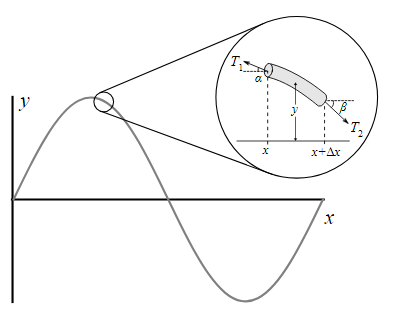
\includegraphics[width=\columnwidth]{fbd.PNG}}
\label{freebody}
\end{figure}



Consider the summation of forces in the $x$ direction:


\begin{equation}
\sum F_x = -T_1 cos(\alpha) + T_2 cos(\beta) = 0
\end{equation}

By definition of this problem, we limit the vibrations to be very small in amplitude whereas we may consider $cos(\alpha) \approx cos(\beta)$ and therefore this equation is satisfied. We now consider the summation of forces in the $y$ direction:

\begin{align}
\sum F_y = T_1sin(\alpha) - T_2sin(\beta) &= \Delta ma\\
T_1sin(\alpha) - T_2sin(\beta) &= \mu \Delta x \frac{d^2y}{dt^2}
\end{align}

Dividing both sides by $T$ and considering $T_1 \approx T_2 \approx T \approx Tcos(\alpha) \approx Tcos(\beta)$ due to the very small angle assumption of $\alpha$ and $\beta$ we can write:

\begin{align}
\frac{Tsin(\alpha)}{Tcos(\alpha)} - \frac{Tsin(\beta)}{Tcos(\beta)} &=  \frac{\mu \Delta x}{T} \frac{d^2y}{dt^2}\\
tan(\alpha) - tan(\beta) &=  \frac{\mu \Delta x}{T} \frac{d^2y}{dt^2}
\end{align}

We can recognize from the free-body diagram that $tan(\alpha)$  and $tan(\beta)$ are simply:

\begin{align}
tan(\alpha) &= \frac{dy}{dx} \Big|^x\\
tan(\beta) &= \frac{dy}{dx} \Big|^{x+\Delta x}
\end{align}

So then:

\begin{align}
 \frac{1}{\Delta x} \Big( \frac{dy}{dx} \Big|^x - \frac{dy}{dx} \Big|^{x+\Delta x}\Big) &=  \frac{\mu}{T} \frac{\partial^2 y}{\partial t^2}
\end{align}

The left hand side is by definition the second derivative of $y$ as $\Delta x$ approaches $0$, and therefore:
\begin{align}
\frac{\partial^2 y}{\partial x^2} = \frac{\mu}{T} \frac{\partial^2y}{\partial t^2}
\end{align}

Or we can replace the constant terms by a single constant:
\begin{align} \label{PDE}
\frac{\partial^2 y}{\partial x^2} = \frac{1}{v^2} \frac{\partial^2y}{\partial t^2}   
\end{align}

Where the wave velocity:
\begin{align}
v = \sqrt{\frac{T}{\mu}}
\end{align}

\subsection{\label{sec:level1}General Solution of the Partial Differential Equation}
The PDE will be solved by the method of separation of variables. The analytical solution for the boundary conditions available will be solved using a Fourier series expansion. We separate the variables and substitute $y(x,t) = X(x)T(t)$ into (\ref{PDE})  and divide by $XT$:

\begin{align}
\frac{1}{X} \frac{\partial^2 X}{\partial x^2} &=  \frac{1}{v^2} \frac{1}{T}\frac{\partial^2T}{\partial t^2}   
\end{align}
The left hand side (LHS) and right hand side (RHS) of this equation are equal and only dependent on their respective variables, $x$ and $y$, respectively. Therefore they must be equal to the same constant, which we will define as $-k^2$ in order to successfully solve the PDE. Therefore:
\begin{align}
\frac{1}{X} \frac{\partial^2 X}{\partial x^2} &= -k^2 \\
\frac{1}{v^2} \frac{1}{T}\frac{\partial^2T}{\partial t^2}  &= -k^2
\end{align}

These two equations can be rearranged to solve for two linear differential equations:

\begin{align}
0 &= X'' + k^2 X \label{XXX}\\\
0 &= T'' + k^2v^2 T \label{YYY}
\end{align}

To solve (\ref{XXX}) we consider the general solution of a second order ODE:

\begin{align}
X(x) &= C_1e^{r_1 x} + C_2e^{r_2 x}
\end{align}

Solving for roots $r_1$ and $r_2$ of the characteristic equation we find that there are only complex roots with no real part, thus:

\begin{align}
X(x) &= c_1 cos(kx) + c_2sin(kx)
\end{align}

We solve $T(t)$ in a similar fashion and find:

\begin{align}
T(t) &= c_3 cos(kvt) + c_4sin(kvt)
\end{align}

Then our general solution of y(x,t) is:

\begin{multline}
y(x,t) =(c_1 cos(kx) + c_2sin(kx))\\(c_3 cos(kvt) + c_4sin(kvt))
\end{multline}

\subsection{\label{sec:level1}Boundary Conditions and Fourier Series Solution}

The first boundary condition to consider is $y(0,t)=y(\ell,t)=0$. This represents the two fixed points at each end of the string. The second condition to consider is the string's initial $y$ velocity $y'(x,0)=y'(x,0)=0.$\\

The final condition required to solve is the initial shape of the "pluck" of the string at rest at $t=0$ as shown in Figure (\ref{boundary}). This "pluck" can be described by a function $y(x,0)$, where we can note that $y(0,0)=y(\ell,0)=0$ :

\begin{figure}[h]
\caption{Initial Condition}
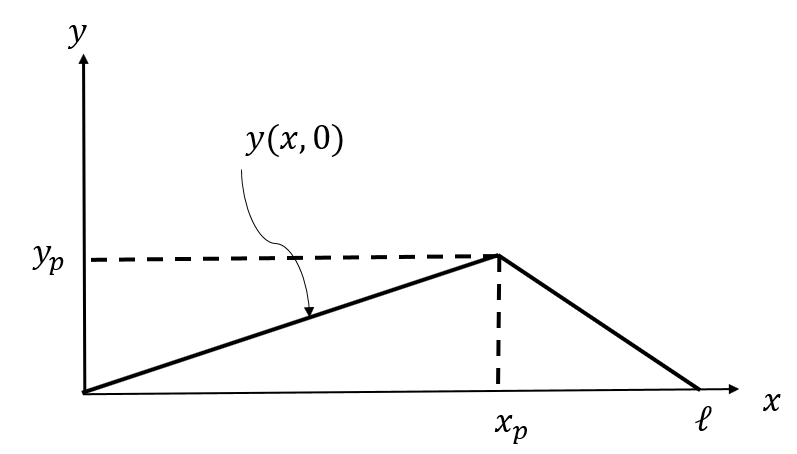
\includegraphics[width=\columnwidth]{boundary.png}
\label{boundary}
\end{figure}

\begin{align} \label{y0}
y(x,0) =  
   \begin{cases} 
      \frac{y_p}{x_p}x & 0 \leq x\leq x_p \\
      \frac{y_p}{\ell-x_p}(\ell-x) & x_p \leq x\leq \ell \\
   \end{cases}
\end{align}

With the boundary condition $y(0,t)=y(\ell,t)=0$, we can solve directly that $c_1 = 0$, leaving (\ref{c2c3c4}). We then consider the derivate (\ref{yprime})  and the second boundary condition mentioned above:

\begin{align}
y(x,t) &=(c_2sin(kx))(c_3 cos(kvt) + c_4sin(kvt)) \label{c2c3c4}\\
y'(x,t) &= (kc_2sin(kx))(kvc_3cos(kvt)+kvc_4sin(kvt)) \label{yprime}
\end{align}

Applying $y'(x,0)=0$ to (\ref{yprime}) we can solve directly that $c_4 = 0$. We can combine arbitrary constants $c_2$ and $c_3$ as shown in (\ref{last}) to be $b$ (\ref{next}).

\begin{align}
y(x,t) &=(c_2sin(kx))(c_3 cos(kvt)) \label{last}\\
y(x,t) &= b sin(kx)cos(kvt) \label{next}
\end{align}

We can recognize that the this equation still has two arbitrary constants to solve for. If we consider $y(x,t)$ as a summation of terms $n$ where $b = \sum_{n=1}^{\infty} b_n$ and define the constant $k = \frac{n\pi}{\ell}$ we can evaluate the function as a series:

\begin{align}
y(x,t) &= \sum_{n=1}^{\infty} b_n sin\Big(\frac{n\pi}{\ell}x\Big)cos\Big(\frac{n\pi v}{\ell}t\Big) \label{yxt}
\end{align}

The equation in this form is recognizable as a Fourier series expansion. For a Fourier series expansion of an odd function (as which we will define our fuction if it were extended leftwards beyond the y-axis), coefficient $b_n$ can be calculated by:

\begin{align}
b_n &= \frac{2}{\ell} \int_{0}^{\ell} f(x)sin\Big(\frac{n\pi}{\ell}x\Big) \label{bngen}
\end{align}

Evaluating (\ref{yxt}) at $t=0$ and then solving for $b_n$ using (\ref{bngen}) where $f(x) = y(x,0)$ (\ref{y0}):

\begin{align}
b_n &= \frac{2y_p\ell sin\Big(\frac{n \pi x_p}{\ell}\Big)}{\pi^2 n}\Big(\frac{1}{x_p} + \frac{1}{\ell-x_p}\Big)
\end{align}

Then finally the analytical solution for $y(x,t)$ is:

\begin{multline}
y(x,t) =\sum_{n=1}^{\infty} \frac{2y_p\ell sin\Big(\frac{n \pi x_p}{\ell}\Big)}{\pi^2 n}\Big(\frac{1}{x_p} + \frac{1}{\ell-x_p}\Big) \\ sin\Big(\frac{n\pi}{\ell}x\Big)cos\Big(\frac{n\pi v}{\ell}t\Big) \label{yxtfinal}
\end{multline}

\section{\label{sec:level1}Implementation}

A computer program was written using the \texttt{Python} programming langauge to plot the solution of $y(x,t)$ and observe how changing various parameters affects the function.\\

The program \texttt{Bow.py} defines an object class \texttt{bow} which generates a "bow" or "string" object from the parameters given (i.e. string length, linear density, pluck height, etc.). The \texttt{bow} class includes various additional functions which can graph the waveform, initial condition, fourier coefficients $b_n$, among others. Furthermore there is a function which writes the strings waveform at the specified pickup location to a \texttt{.wav} file, and another that generates the Fast Fourier Transform (FFT) of the waveform. \\

A set of test demonstrations numbered 1 through 5 are hard coded at the end of \texttt{Bow.py} to demonstrate the impact of changing various parameters on $y(x,t)$. These test demonstrations are discussed in the following sections.\\ 

As an additional recreational exercise, the program generates sets of audio samples representative of the 88 keys of a piano, and the first 12 frets of a guitar. These samples have been compiled into Ableton Live "Sampler" devices which can be used to play the samples with a MIDI keyboard or \texttt{.mid} file.\\

\section{\label{sec:level1}Discussion}



\subsection{\label{sec:level1}Tension, Density, Length, and Frequency}
The relationship between tension, density, string length, and frequency are correlated independently of the solution of $y(x,t)$, and can be expresed as such with a single expression. We can write the two following expressions for wave velocity $v$:

\begin{align}
v &= \sqrt{\frac{T}{\mu}}\\
v &= f \lambda
\end{align}

Therefore in terms of frequency $f$ and with $\lambda = 2 \ell$:

\begin{align} \label{duh}
f = \frac{1}{2\ell} \sqrt{\frac{T}{\mu}}
\end{align}

\begin{figure}[h]
\caption{Test 1}
\fbox{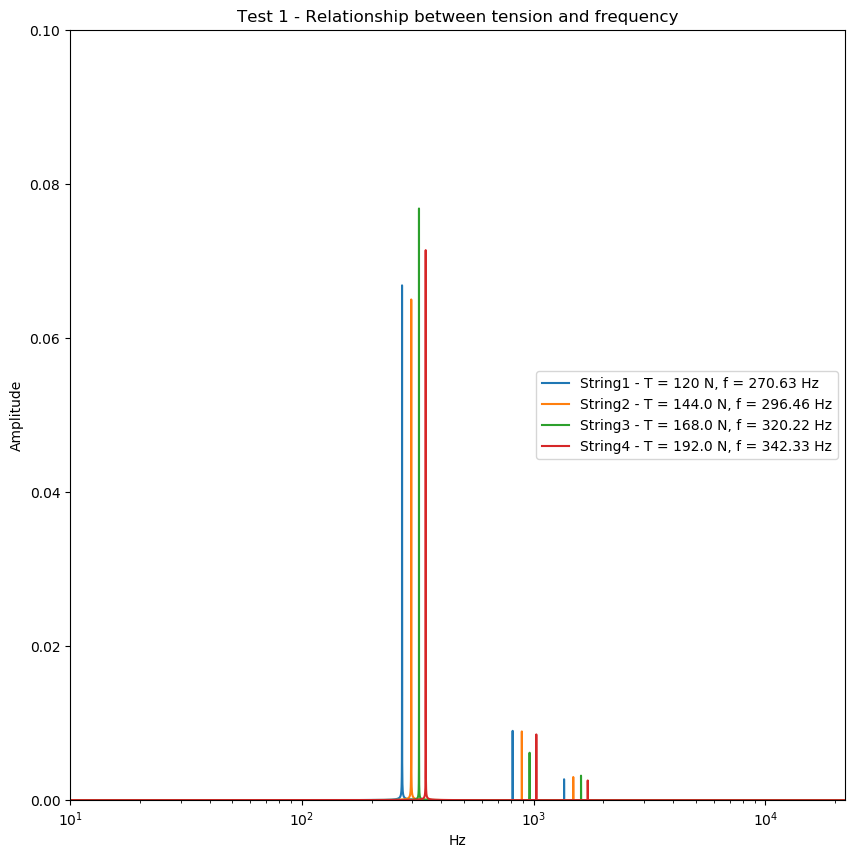
\includegraphics[width=\columnwidth]{Test1_T_vs_freq.png}}
\label{Test1}
\end{figure}

\begin{figure}[h]
\caption{Test 2}
\fbox{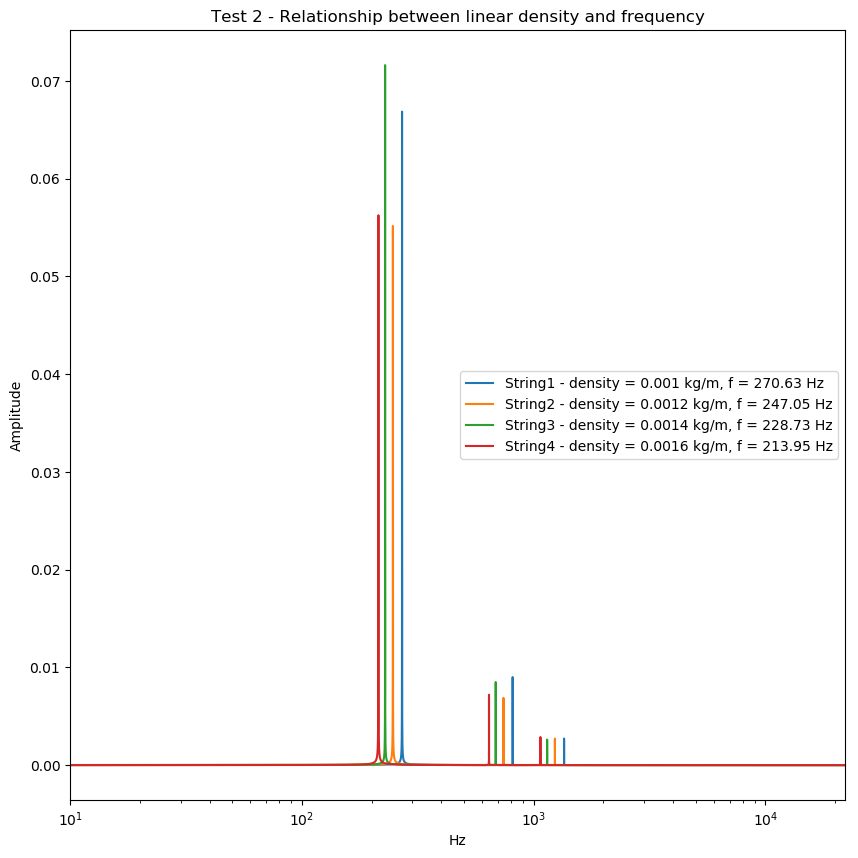
\includegraphics[width=\columnwidth]{Test2_density_vs_freq.png}}
\label{Test2}
\end{figure}

\begin{figure}[h]
\caption{Test 3}
\fbox{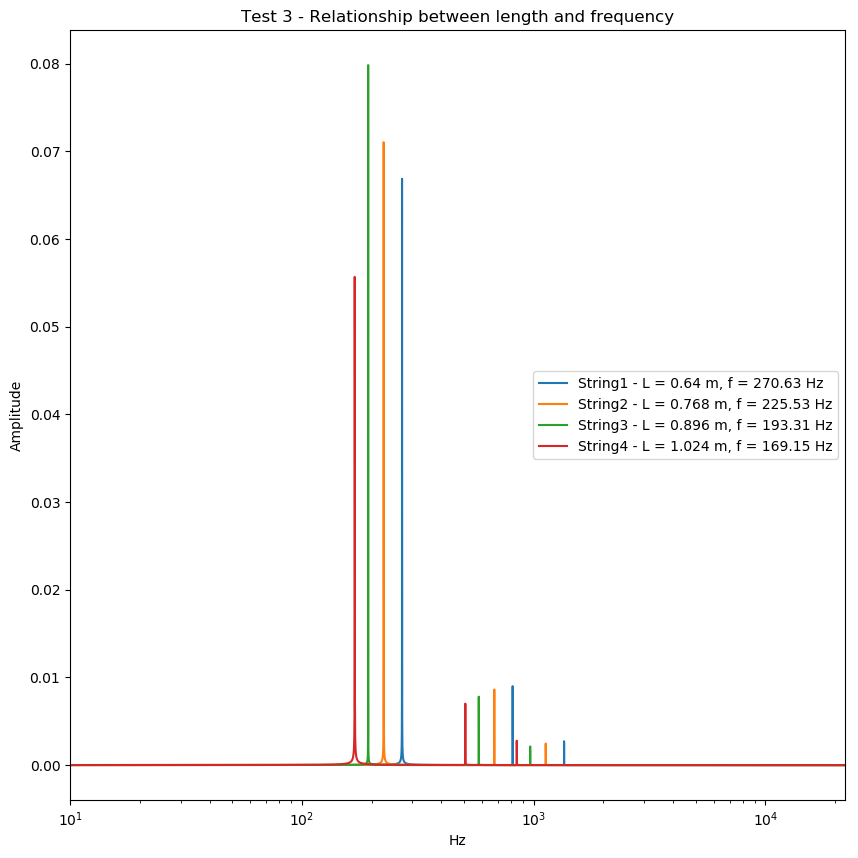
\includegraphics[width=\columnwidth]{Test3_length_vs_freq.png}}
\label{Test3}
\end{figure}

Figures \ref{Test1}, \ref{Test2}, and \ref{Test3} show three frequency spectrums of the same "string" with various parameters being changed, and their resulting frequency response. Test 1 demonstrates that increasing the tension of the string will increase the frequency. Test 2 demonstrates that increasing the linear density will decrease the frequency. Test 3 demonstrates that increasing the string length will decrease the frequency. All these relationships are straightforward when considering (\ref{duh}).\\

The physical properties used to define the string are $\ell = 0.640$ m, $T = 120$ N, $\mu = 0.001$ kg/m. 





\subsection{\label{sec:level1}Sound Pick-up Location}

Changing the sound pick-up location $x_pup$ changes the frequency response of the sound wave as well. This is analagous to how an electric guitar may have two or three electromagnetic pick-ups, located in different places on the body of the guitar along the strings. Typically the bridge pick-up near the end of the strings has more "treble" (higher frequencies) and the neck pick-up closer to the center point of the strings has more "bass" (lower frequencies). This relationship was investigated using the solution of $y(x,t)$.\\

When $x = x_{pup}$, the $sin$ term in (\ref{yxtfinal}) becomes dependent only on integer variable $n$. Therefore by changing where the sound pick-up "listens" to the string, the fourier coefficients $b_n$ are then multiplied by this new constant term, and therefore affects the frequencies present in the sound wave. \\

Changing the location of $x_{pup}$ between $ 0 < x_{pup} <\ell$ changes the value of the argument of the $sin$ function. One can notice that at the very center of the string when $x = x_{pup} = \frac{\ell}{2}$, the sin term becomes $sin(\frac{n \pi}{2})$, and therefore the $sin$ term becomes either -1, 0, or 1, which eliminates half of all series expansion terms. For all other values of $x_{pup}$, the sin term can be any value between -1 and 1, and therefore additional sound harmonics may be present.\\

The four frequency response spectrums shown in Figure \ref{Test4} show how the harmonics present in a wave can change depending where the sound pick-up is. It is evident that when $x = x_{pup} = \frac{\ell}{2}$ the fewest upper harmonics are present.
 
\begin{figure}[h]
\caption{Test 4}
\fbox{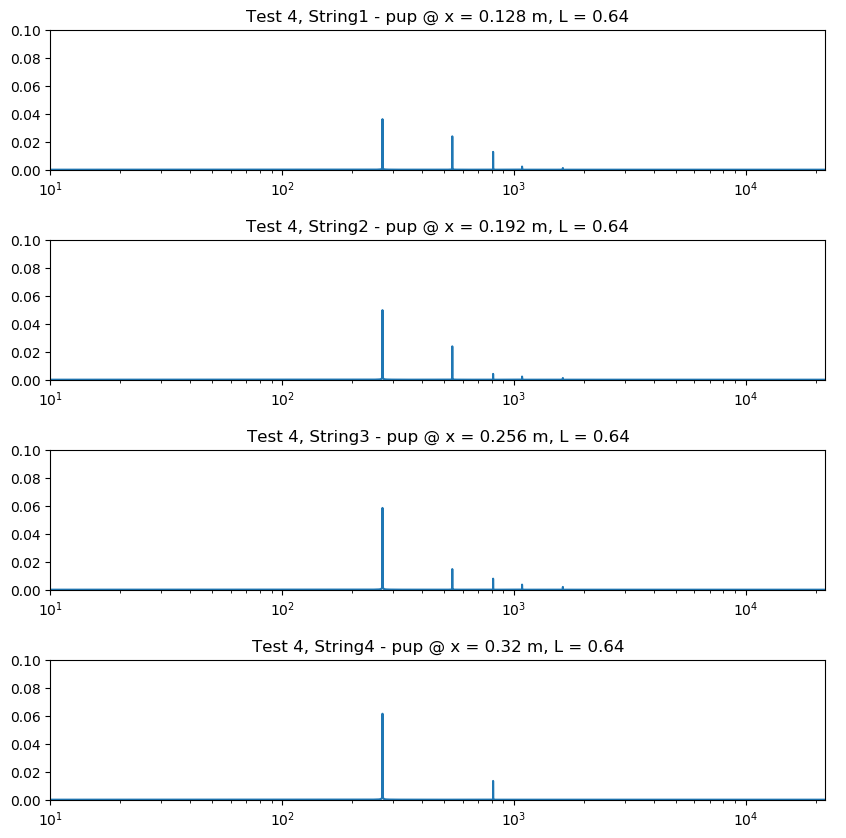
\includegraphics[width=\columnwidth]{Test4_pickup.png}}
\label{Test4}
\end{figure}

\subsection{\label{sec:level1}Sound Pluck Location}

In a similar fashion to changing the sound pick-up location, changing the pluck location can also affect the frequency content, when considering a constant pick-up location. \\
\begin{figure}[h]
\caption{Test 5}
\fbox{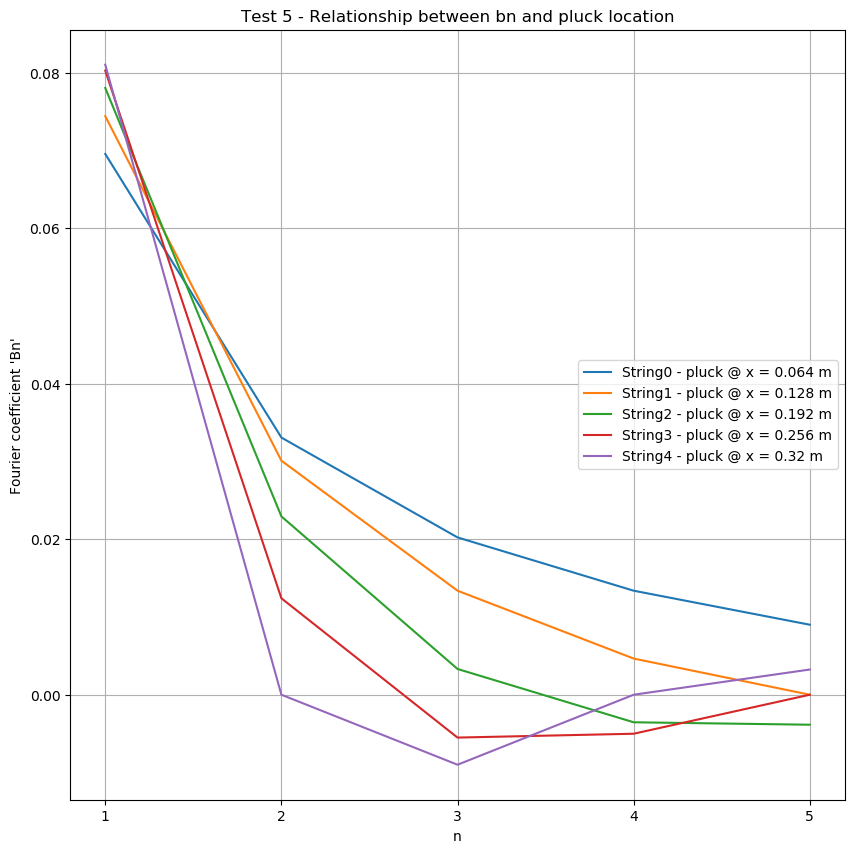
\includegraphics[width=\columnwidth]{Test5_bn_vs_xp.png}}
\label{Test5}
\end{figure}
When $x = x_{pup}= $ constant, it can be seen that the constant term of (\ref{yxtfinal}) is dependent only on $x_p$. Similarly to the sound pick-up location discussed above, the $sin$ term in $b_n$becomes $sin(\frac{n \pi}{2})$ when  $x_{p} = \frac{\ell}{2}$, and half of all series expansion terms are eliminated.

For values of $x_p/\ell \neq 1/2$, all series expansion terms are present. As $x_p/\ell$ strays futher from the midpoint and approaches 0 or 1, the harmonic content (comparatively, Fourier coefficients $b_n$) increase. This is shown in Figure \ref{Test5} for the first nine $n$.



\section{\label{sec:level1}Future Work}

Two additional areas of particular interest or future study and implementation are as follows:\\

\begin{enumerate}
  \item Use solution of $y'(x,0)$ as the initial condition to model/simulate the string being struck and inducing a velocity profile across the string. This would allow the generated waveform to have a solution where $y(x,0)=0$. This would be a nice improvement for sound sample generation as the current program because when the generated \texttt{.wav} file that is currently generated is played in an audio device, a "click" is heard as the speakers try to quickly move as a step change to $y(x_{pup},0)$.
  \item The model currently does not consider any damping from air resistance or vibrational energy loss at the two fixed ends. Implementation of either of these damping models would be interesting as the generated waveform may then include an amplitude and/or frequency envelope. 
\end{enumerate}

\section{\label{sec:level1}Conclusion}
In conclusion this project has ultimately satisfied the author's curiosity. The mathematical model and computer program written to simulate an undampened vibrating string has demonstrated how the pick-up location and pluck location can affect the frequency content of the resulting soundwave.\\

\section{\label{sec:level1}Source Code}
The \texttt{Python} code, graphics, generated \texttt{.wav} files, and Ableton Live set (.als) file with Sampler devices are hosted on GitHub at the following URL: 
\url{https://github.com/jeastick/ENGR-5696/tree/master/Project}




























\end{document}
%
% ****** End of file apssamp.tex ******